%\documentclass[preprint, review, 3p, authoryear]{elsarticle}
\documentclass[10pt, a4paper]{article}

%\usepackage{setspace}
\usepackage[utf8]{inputenc}
\usepackage{amsmath, amssymb, amsthm, bbm}
\usepackage{xcolor}
\usepackage{graphicx}
\usepackage[authoryear]{natbib}
\usepackage{apalike}

\DeclareMathOperator*{\argmax}{arg\,max}

\newtheorem{prob}{Problem}
\newtheorem{prop}{Proposition}
\newtheorem{definition}{Definition}

%%%%% bold symbol in math enviornment
\newcommand{\m}[1]{\boldsymbol{#1}}

\title{Merging Gaussian mixtures using  posterior probabilities}
\author{M. Comas-Cufí \and J.A. Martín-Fernández \and G. Mateu-Figueras}

%\doublespacing
\begin{document}

\maketitle

\section{Introduction}

Different he problem of merging the components of a Gaussian mixtures has received special atention \cite{melnykov2013distribution,lee2004combining,hennig2010methods,baudry2010combining,pastore2013merging}. 

In general, \cite{hennig2010methods} summarises the algorithm of hierarchically merging Gaussian components as follows:
\begin{enumerate}
\item Start with all components of the initially estimated Gaussian mixture as current clusters
\item Find a pair of components to merge and forming a single cluster
%\item Calculate the posterior probability of pertinence to a cluster 
\item Apply a stopping criterion to decide whether to merge them to form a new current cluster, or to use the current clustering as the final one.
\item If merged, go to 2.
\end{enumerate}

In this paper we focus on methods based on misclassification probabilities. Concretely, on those depending on the posterior probabilities \citep{melnykov2013distribution}, \citep{baudry2010combining} and \citep[in \textsc{demp} approach]{hennig2010methods}. Our aim is to find strategies to hierachically merge components into clusters. In this article, for the different strategies we will not focus on stopping criteria, and therefore we will hierarchically merge all components until un sigle cluster with all the components is obtained.


We exposes the problem in a general setting which contains the approaches proposed by Baudry and Hennig.

% \section{The subjectiveness of clustering decisions}
% 
% It is well known that there is a strong subjective component in the decision of what a ``true cluster'' is \citep{hennig2010methods}.
%
% \begin{prob}
% Given a compositional sample $T = \{ \boldsymbol{\tau_1}, \dots, \boldsymbol{\tau_n} \}$, with $\boldsymbol{\tau_i} = (\tau_{i1}, \dots, \tau_{iK})$ denoting the pertinence to classes $C_1, \dots, C_K$, build a hierarchy over the set of classes.
% \end{prob}

\section{Definitions}
\label{definitions}

Let $\mathbb{X}$ be a sample space. A \emph{finite mixture of distributions} is a probability distribution with a pdf defined as the linear combination of pdf from other probability distributions, all defined in $\mathbb{X}$. In general, the pdf $f$ of a finite mixture of distributions is
\begin{equation}\label{mixt}
f(\;\cdot\; ; \pi_1, \dots, \pi_k, \m\theta_1 \dots \m\theta_k) = \pi_1 f_1(\;\cdot\; ; \m\theta_1) + \dots + \pi_k f_k(\;\cdot\; ; \m\theta_k),
\end{equation}
where $\m\theta_1, \dots,  \m\theta_k$ are the parameters of the pdf $f_1, \dots, f_k$ respectively and, because $f$ is a pdf, we have the restriction $\sum_{\ell = 1}^k \pi_\ell = 1$. The probability distributions $f_j$, $1 \leq j \leq k$, are called the \emph{components} of the finite mixture $f$, or \emph{mixture components}.

Let $f$ be finite mixture of distributions as defined in Equation~\ref{mixt} with  parameters  $\pi_1, \dots, \pi_k, \m\theta_1 \dots \m\theta_k$ and let $I$  be a subset of $\{1, \dots, k\}$. We denote by $f_I$ the finite mixture of distributions with pdf defined by
\[
f_I = \sum_{j \in I} \frac{\pi_i}{\pi_I} f_j(\;\cdot\; ; \m\theta_j)
\]
where $\pi_I = \sum_{\ell \in I} \pi_\ell$. To simplify, we do not specify the parameters of $f_I$, which are parameters borrowed from $f$. Note that using this notation, we have that $f_{\{1, \dots, k\}} = f$ and $f_{\{j\}} = f_j$.

A \emph{partition} $\mathcal{I}$ of $\{1, \dots, k\}$ is a set of subsets of $\{1, \dots, k\}$, called $parts$, such that $\bigcup_{I \in \mathcal{I}} I = \{1, \dots, k\}$ and  if two parts $I$, $J$ are different, $I \cap J = \emptyset$ holds. To simplify, through this paper we assume an order within the elements of a partition. Doing so, we can index the partition and write $\mathcal{I} = \{ I_1, \dots, I_s\}$. Note that for any partition $\mathcal{I} = \{ I_1, \dots, I_s\}$ the mixture $f$ can be rewritten as:
\[
f = \pi_{I_1} f_{I_1} + \dots + \pi_{I_s} f_{I_s}.
\]


A \emph{hierarchical combination of components} is a sequence of partitions $\mathcal{I}_1, \dots, \mathcal{I}_k$ of $\{1,...,k\}$, where $\mathcal{I}_1$ is the one-part partition $\mathcal{I}_1 = \{ \{1, \dots, k\} \}$, and for each $k'$, $1 <  k' \leq k$,
\begin{itemize}
\item $\mathcal{I}_{k'}$ has $i$ elements  and
\item if a part $I \in \mathcal{I}_{k'-1}$ then there is a part $J \in \mathcal{I}_{k'}$ with $J = I$ or there are two parts $J_1, J_2 \in \mathcal{I}_i$ with $I = J_1 \cup J_2$.
\end{itemize}


\subsection*{Model-based clustering}

When model-based clustering is based on finite mixtures, a common approach is to assume that a sample is following a finite mixture of distributions $f_1, \dots, f_k$, and then proceed as follows, 
\begin{enumerate}
\item find a suitable estimators $\hat{\pi}_1, \dots, \hat{\pi}_k, \hat{\m\theta}_1, \dots, \hat{\m\theta}_k$ of parameters $\pi_1, \dots, \pi_k, \m\theta_1, \dots, \m\theta_k$, and
\item to classify each observation according to the maximum a posteriori criteria, i.e., two observations $\m x, \m y \in \mathbb{X}$ are classified to same cluster if and only if
\[
\argmax_{j=1}^k \frac{ \hat{\pi}_j f_j(\m x ; \hat{\m\theta}_j) }{\sum_{\ell=1}^k \hat{\pi}_\ell f_\ell(\m x ; \hat{\m\theta}_\ell) } = \argmax_{j=1}^k \frac{ \hat{\pi}_j f_j(\m y ; \hat{\m\theta}_j) }{ \sum_{\ell=1}^k \hat{\pi}_\ell f_\ell(\m y ; \hat{\m\theta}_\ell) }.
\]
\end{enumerate}


\cite{lee2004combining,hennig2010methods,baudry2010combining,melnykov2013distribution,pastore2013merging} noted that classifying an element according to the probability of belonging to one component could be misleading. Instead, they propose that one cluster can be formed by the combination of different components. Formally, given a partition $\mathcal{I} = \{ I_1, \dots, I_s\}$, two elements $\m x, \m y \in \mathbb{X}$ are classified to the same cluster if and only if
\[
\argmax_{j=1}^s \frac{ \hat{\pi}_{I_j} \hat{f}_{I_j}(\m x) }{\sum_{\ell=1}^s \hat{\pi}_{I_\ell} \hat{f}_{I_\ell}(\m x ) } = \argmax_{j=1}^s \frac{ \hat{\pi}_{I_j} \hat{f}_{I_j}(\m y) }{ \sum_{\ell=1}^s \hat{\pi}_{I_\ell} \hat{f}_{I_\ell}(\m y) }
\]
where $\hat{f}_{I_j}(\; \cdot \;) = \sum_{j' \in I_j} \frac{\hat{\pi}_{j'}}{\hat{\pi}_{I_j}} f_{j'}(\; \cdot \; ; \hat{\m\theta}_{j'})$ and $\hat{\pi}_{I_j} =  \sum_{j' \in I} \hat{\pi}_{j'}$. 

Let $X = \{\m x_1\dots, \m x_n\}$ be a sample in defined in $\mathbb{X}$. Along this paper we define
\[
\hat{\tau}_{i I_j} =  \frac{ \hat{\pi}_{I_j} \hat{f}_{I_j}(\m x_i) }{\sum_{i=1}^k \hat{\pi}_{I_j} \hat{f}_{I_j}(\m x_i)},
\]
and, for a partition  $\mathcal{I} = \{ I_1, \dots, I_s\}$, we define
\[
\hat{\tau}_{i \mathcal{I}} = \left( \hat{\tau}_{i I_1} , \dots, \hat{\tau}_{i I_s}  \right).
\]
Note that whenever  $\mathcal{I} = \{ I_1, \dots, I_s\}$ is a partition, $\sum_{j=1}^s \hat{\tau}_{i I_j} = 1$ for $1 \leq i \leq n$.

For the sake of an example, consider following  estimated Gaussian mixture

\[
\hat{f} = \sum_{j=1}^6 \hat{\pi}_j \phi(\;\cdot\; ; \hat{\m\mu}_j, \hat{\m\Sigma}_j)
\]
with parameters
{\small
\[
\begin{array}{l@{\hskip 0.1in}l@{\hskip 0.1in}c }
\hat{\pi}_1 = 0.13, & \hat{\m\mu}_1 = \left(10.8,69.17\right), & \hat{\m\Sigma}_1 = \left(
\begin{array}{cc}
36.41&1.45 \\ 
1.45&55.13 \\ 
\end{array}
\right), \\ & &\\ 
\end{array}
\]
\[
\begin{array}{l@{\hskip 0.1in}l@{\hskip 0.1in}c }
\hat{\pi}_2 = 0.09, & \hat{\m\mu}_2 = \left(32.68,22.46\right), & \hat{\m\Sigma}_2 = \left(
\begin{array}{cc}
26.76&1.07 \\ 
1.07&40.52 \\ 
\end{array}
\right), \\ & &\\ 
\end{array}
\]
\[
\begin{array}{l@{\hskip 0.1in}l@{\hskip 0.1in}c }
\hat{\pi}_3 = 0.07, & \hat{\m\mu}_3 = \left(13.65,51.91\right), & \hat{\m\Sigma}_3 = \left(
\begin{array}{cc}
33.95&1.35 \\ 
1.35&51.39 \\ 
\end{array}
\right), \\ & &\\ 
\end{array}
\]
\[
\begin{array}{l@{\hskip 0.1in}l@{\hskip 0.1in}c }
\hat{\pi}_4 = 0.16, & \hat{\m\mu}_4 = \left(83.8,4.21\right), & \hat{\m\Sigma}_4 = \left(
\begin{array}{cc}
82.27&3.28 \\ 
3.28&124.56 \\ 
\end{array}
\right), \\ & &\\ 
\end{array}
\]
\[
\begin{array}{l@{\hskip 0.1in}l@{\hskip 0.1in}c }
\hat{\pi}_5 = 0.24, & \hat{\m\mu}_5 = \left(41.28,19.51\right), & \hat{\m\Sigma}_5 = \left(
\begin{array}{cc}
55.87&2.23 \\ 
2.23&84.59 \\ 
\end{array}
\right), \\ & &\\ 
\end{array}
\]
\[
\begin{array}{l@{\hskip 0.1in}l@{\hskip 0.1in}c }
\hat{\pi}_6 = 0.32, & \hat{\m\mu}_6 = \left(24.69,66.04\right), & \hat{\m\Sigma}_6 = \left(
\begin{array}{cc}
57.85&2.3 \\ 
2.3&87.58 \\ 
\end{array}
\right), \\ & &\\ 
\end{array}
\]

}

Mixture $\hat{f}$ has been estimated using a sample $X_{500}=\{\m x_1, \dots, \m x_{500}\}$ generated by the R package \textsc{MixSim}. The data points in sample $X_{500}$ follows a Gaussian mixture \emph{with 3 components}. The overlapping between components $\omega$ is a measure that defined the overlapping between components in a mixture. To generate sample $X_{500}$ a maximum overlapping of  $\check{\omega} = 0.01$ was fixed (see Melnykov for more details). In Figure~\ref{ex_mixture} the sample is represented with the isodensity curves of the adjusted mixture $\hat{f}$ and the estimated parameter $\hat{\mu}_j$ of each component.

\begin{figure}[thbp]
\begin{center}
\begin{tabular}{cc}
 %   6 toy mixture
  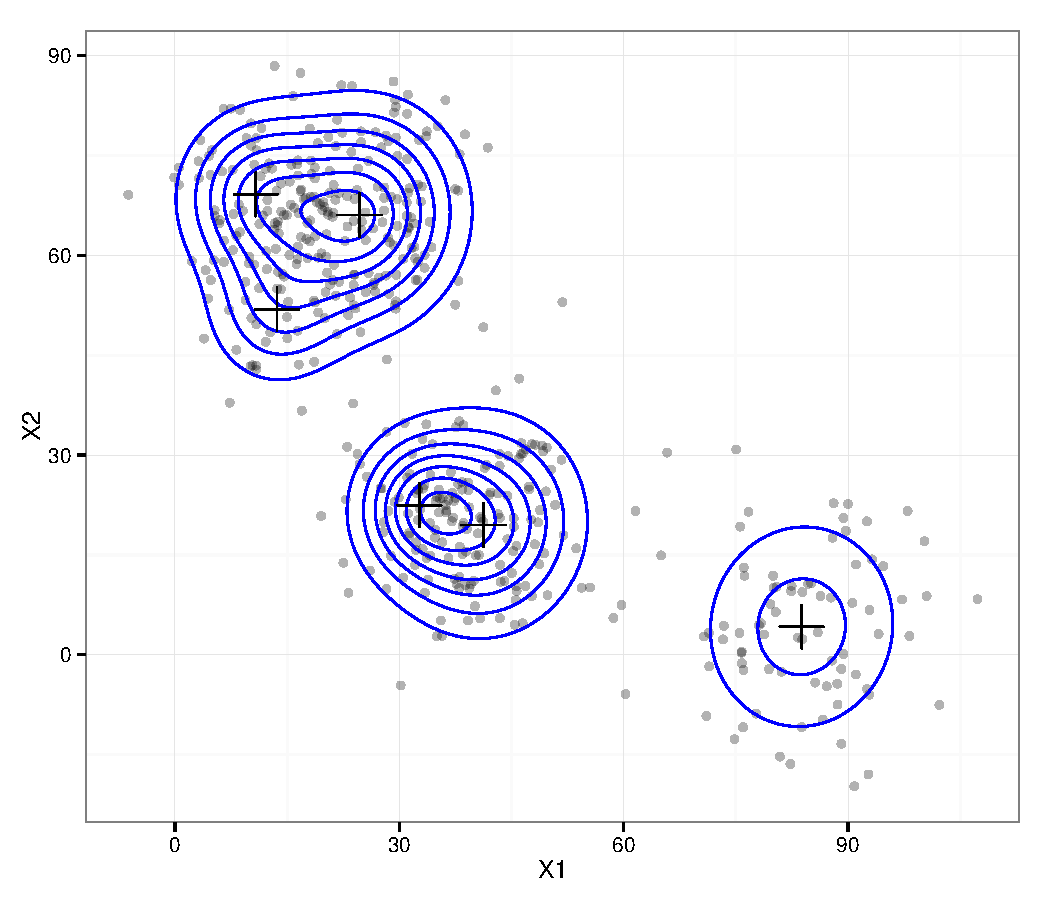
\includegraphics[trim=0cm 0cm 0cm 0cm,width=0.6\textwidth]{figures/partition-example-mixture.pdf} \\
 \end{tabular}
 \caption{Density of a 6 component Gaussian mixture adjusted to a data set generated from a 3 component Gaussian mixture using R \textsc{MixSim} package with max overlapping of $\check{\omega} = 0.01$.}\label{ex_mixture}
\end{center}
\end{figure}

Let $I = \{1,2,3,4,5,6\}$. As commented before, any partition of $I$ yields to a cluster algorithm. For example, consider the partition 
\[\mathcal{I}_6 = \{\{1\},\{2\},\{3\},\{4\},\{5\},\{6\}\}\]
of $I$. Using partition $\mathcal{I}_6$ every observation $\m x_i \in \mathbb{R}^2$ is assigned to the part $\{j\}$ for which $\hat{\tau}_{i\{j\}}$ is maximum. In Figure~\ref{ex_part6} each observation $\m x_i$ has been separated according to the assigned part. Moreover, the isodensity curves for each of the pdf $\hat{f}_{\{j\}} = \phi(\;\cdot\; ; \hat{\m\mu}_j, \hat{\m\Sigma}_j)$, $1\leq j \leq 6$, have also been included in the graphic. 

%In other words, $\m x_i \in \mathbb{R}^2$ is assigned to cluster labeled
%\[
%\argmax_{j=1}^6 \frac{ \hat{\pi}_{\{j\}} \hat{f}_{\{j\}}(\m x) }{\sum_{\ell=1}^6 \hat{\pi}_{I_\ell} \hat{f}_{I_\ell}(\m x ) }
%\]


%$\hat{f}_{\{j\}}(\;\cdot\;) = \frac{\hat{\pi}_j}{\hat{\pi}_j} f(\;\cdot\;; \hat{\m\mu}_j, \hat{\m\Sigma}_j) = f(\;\cdot\;; \hat{\m\mu}_j, \hat{\m\Sigma}_j)$ for $j = 1,...,6$. Partition $\mathcal{I}_6$ yields to the cluster algorithm where an element $x_i$ is assigned to the part $\{j\}$ of $\mathcal{I}_6$ such that $\hat{\tau}_{i\{j\}}$ is maximum.


\begin{figure}[!h]
\begin{center}
\begin{tabular}{cc}
 %   6 toy mixture
  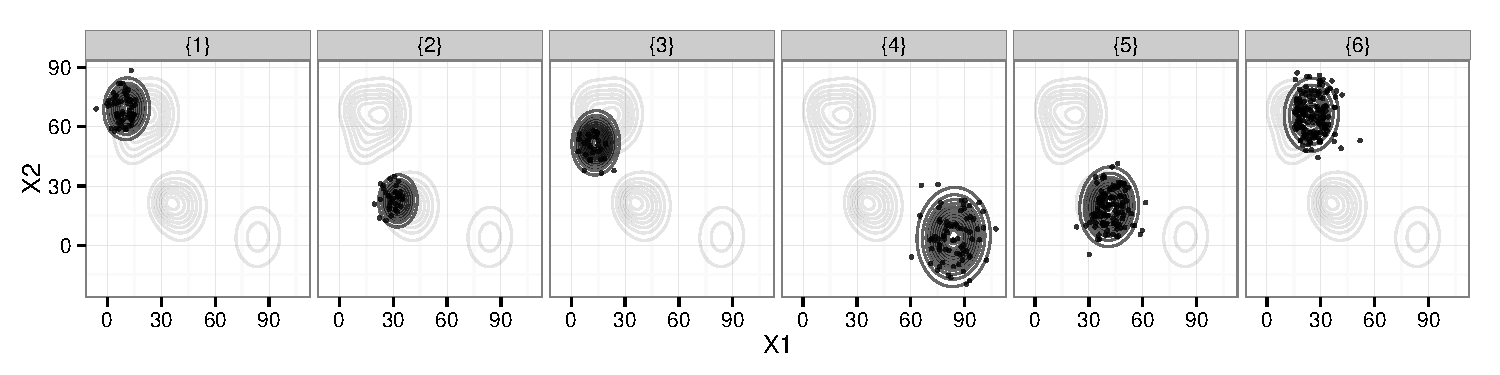
\includegraphics[trim=0cm 0cm 0cm 0cm,width=\textwidth]{figures/partition-example-part6.pdf} \\
 \end{tabular}
 \caption{Classifying assigning each observation to a single component}\label{ex_part6}
\end{center}
\end{figure}

In contrast, if we consider the partition
\[\mathcal{I}_3 = \{\{1, 3, 6\},\{2, 5\},\{4\}\}\]
which is grouping those components with closest mean. We get the 3 clusters given in Figure~\ref{ex_part3a}, where we have included the isodensity curves of pdf $\hat{f}_{\{1,3,6\}}$, $\hat{f}_{\{2, 5\}}$ and $\hat{f}_{\{4\}}$ given by

\[ 
%\left\{ 
\begin{array}{r c l}
\hat{f}_{\{1,3,6\}} & = & \frac{1}{0.52}(0.13 \phi(\;\cdot\; ; \hat{\m\mu}_1, \hat{\m\Sigma}_1) + 0.07 \phi(\;\cdot\; ; \hat{\m\mu}_3, \hat{\m\Sigma}_3) + 0.32 \phi(\;\cdot\; ; \hat{\m\mu}_6, \hat{\m\Sigma}_6)), \\
\hat{f}_{\{2, 5\}} & = &  \frac{1}{0.33}(0.09 \phi(\;\cdot\; ; \hat{\m\mu}_2, \hat{\m\Sigma}_2) + 0.24 \phi(\;\cdot\; ; \hat{\m\mu}_5, \hat{\m\Sigma}_5)), \\
\hat{f}_{\{4\}} & = &\phi(\;\cdot\; ; \hat{\m\mu}_4, \hat{\m\Sigma}_4).
\end{array} 
%\right. 
\]
  


\begin{figure}[!h]
\begin{center}
\begin{tabular}{cc}
  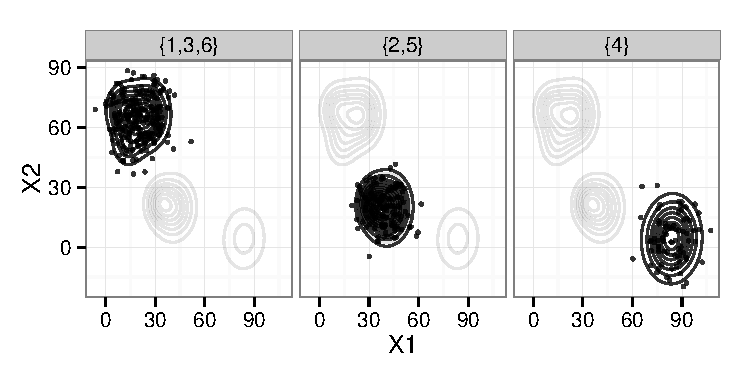
\includegraphics[trim=0cm 0cm 0cm 0cm,width=0.6\textwidth]{figures/partition-example-part3a.pdf} \\
 \end{tabular}
 \caption{Classifying assigning each observation to a single component}\label{ex_part3a}
\end{center}
\end{figure}

Finally, suppose that instead of grouping by similar mean, we decide to group by similar covariance matrix. By choosing partition
\[\mathcal{I}'_3 = \{\{1, 2, 3\},\{4\},\{5, 6\}\},\]
we end up with the clustering given in Figure~\ref{ex_part3b}.

\begin{figure}[!h]
\begin{center}
\begin{tabular}{cc}
  \includegraphics[trim=0cm 0cm 0cm 0cm,width=0.6\textwidth]{figures/partition-example-part3b.pdf} \\
 \end{tabular}
 \caption{Classifying assigning each observation to a single component}\label{ex_part3b}
\end{center}
\end{figure}

Consider the following hierarchical combination of components given by the following sequence
\begin{equation}
\begin{array}{r c c}
\mathcal{H}(\mathcal{I}) &=& \{ \{\{1\},\{2\},\{3\},\{4\},\{5\},\{6\}\}, \\
   & & \{\{1, 6\},\{2\},\{3\},\{4\},\{5\} \}, \\
   & &    \{\{1, 6, 3\},\{2\},\{4\},\{5\} \}, \\
   & &    \{\{1, 6, 3\},\{2\},\{4, 5\} \}, \\
    & &   \{\{1, 6, 3\},\{2, 4, 5\} \}, \\
   & &    \{\{1, 2, 3, 4, 5, 6\}\} \}.
\end{array}
\label{hier_ex}
\end{equation}
we obtain the hierarchical clustering given in Figure~\ref{hierarchical}

\begin{figure}[!h]
\begin{center}
\begin{tabular}{cc}
  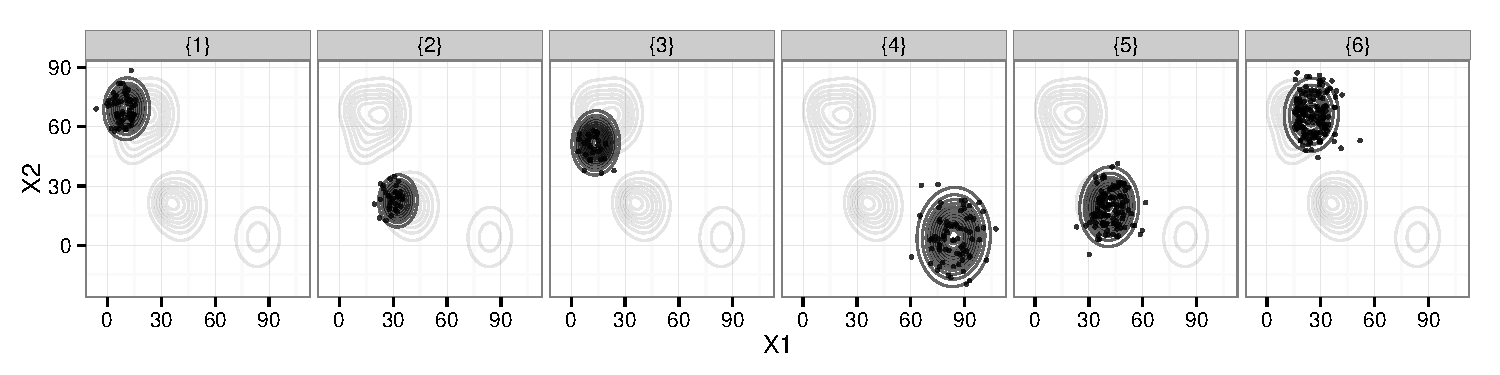
\includegraphics[trim=0cm 0cm 0cm 0cm,width=\textwidth]{figures/partition-example-part6.pdf} \\
    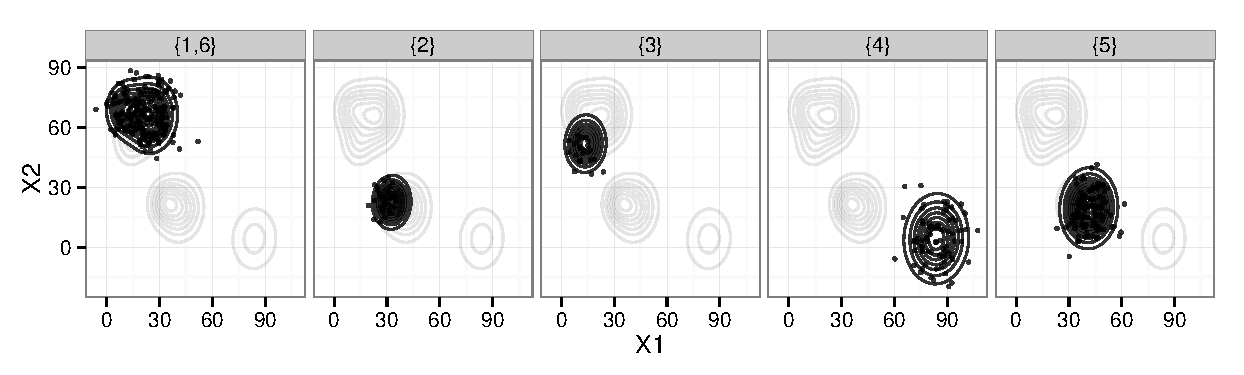
\includegraphics[trim=0cm 0cm 0cm 0cm,width=0.83\textwidth]{figures/partition-example-part5.pdf} \\
      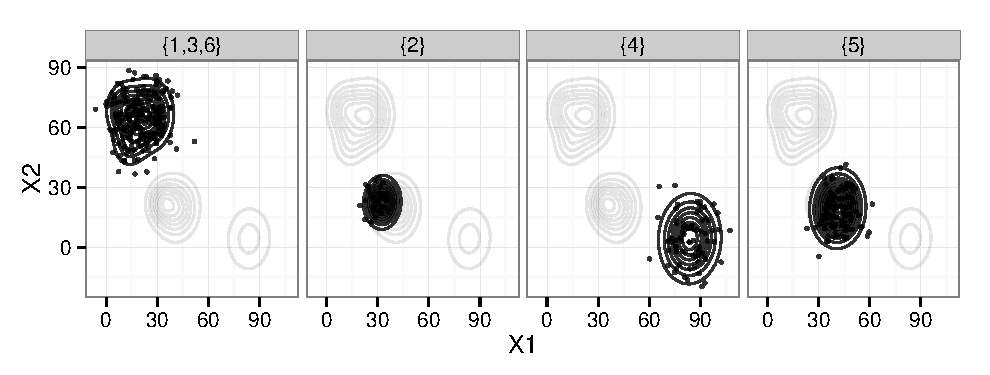
\includegraphics[trim=0cm 0cm 0cm 0cm,width=0.67\textwidth]{figures/partition-example-part4.pdf} \\
        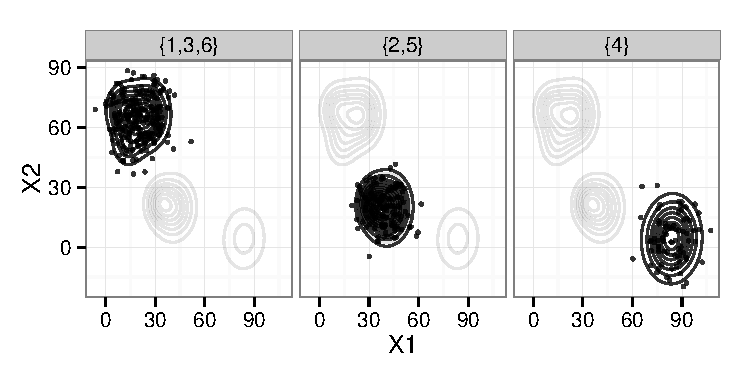
\includegraphics[trim=0cm 0cm 0cm 0cm,width=0.5\textwidth]{figures/partition-example-part3a.pdf} \\
          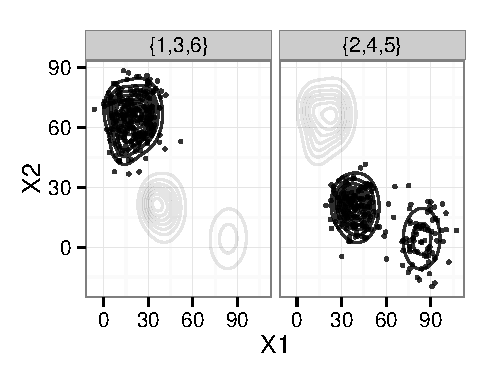
\includegraphics[trim=0cm 0cm 0cm 0cm,width=0.33\textwidth]{figures/partition-example-part2.pdf} \\
            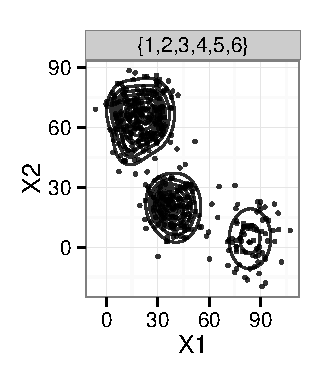
\includegraphics[trim=0cm 0cm 0cm 0cm,width=0.17\textwidth]{figures/partition-example-part1.pdf}
 \end{tabular}
 \caption{Hierarchical cluster obtained by the hierarchical combination of components given in Eq.~\ref{hier_ex}.}\label{ex_part3a}
\end{center}
\end{figure}

\section{Hierarchical algorithms based on posterior probabilities}

Using definitions given in Section~\ref{definitions} we revisite some Hierarchical algorithms based on posterior probabilities

\subsection*{Algorithm based on the total Entropy}

%Let ${\boldsymbol\tau}_1, \dots, {\boldsymbol\tau}_n$ be the probability vectors giving the probability that elements $\textbf{x}_1, \dots, \textbf{x}_n$ belongs to classes $C_1, \dots, C_k$.  

\cite{baudry2010combining} proposes the  hierarchical combination of components  $\mathcal{I}_1 \dots, \mathcal{I}_k$ defined as follows: starting from partition $\mathcal{I}_k = \{\{1\},\dots, \{k\}\}$ at each step the method combine two parts. If at current step we have the partition  $I_1, \dots, I_s$ the two parts, $I_a, I_b$, $1 \leq a,b \leq s$, to be combined are those that maximise the entropy criterion

\[
- \sum_{i=1}^n \left\{ \hat{\tau}_{iI_a} \log(\hat{\tau}_{iI_a}) + \hat{\tau}_{iI_b} \log(\hat{\tau}_{iI_b})\right\} +  \sum_{i=1}^n  (\hat{\tau}_{iI_a}+\hat{\tau}_{iI_b}) \log(\hat{\tau}_{iI_a} + \hat{\tau}_{iI_b}),
\]

or equivalently,

\[
 \sum_{i=1}^n \hat{\tau}_{i I_a \cup I_b} \log(\hat{\tau}_{i I_a \cup I_b}) - \hat{\tau}_{iI_a} \log(\hat{\tau}_{iI_a}) - \hat{\tau}_{iI_b} \log(\hat{\tau}_{iI_b}).
\]

%in other words $\dots$

\subsection*{DEMP algorithm}

%Let ${\boldsymbol\tau}_1, \dots, {\boldsymbol\tau}_n$ be the probability vectors giving the probability that elements $\textbf{x}_1, \dots, \textbf{x}_n$ belongs to classes $C_1, \dots, C_k$. 

DEMP approach \citep{hennig2010methods} proposes the hierarchical combination of components  $\mathcal{I}_1 \dots, \mathcal{I}_k$ defined as follows: starting from partition $\mathcal{I}_k = \{\{1\},\dots, \{k\}\}$ at each step the method combine two parts. If at current step we have the partition  $I_1, \dots, I_s$ the two parts, $I_a, I_b$, $1 \leq a,b \leq s$,  to be combined are those that maximise the misclassification probabilities estimated by 

\[
\frac{ \frac{1}{n} \sum_{i=1}^n {\hat{\tau}_{iI_a} \mathbbm{1}_{\left[ \forall j\; \hat{\tau}_{i I_{b}} \geq \hat{\tau}_{iI_j} \right]}}}{ \hat{\pi}_{I_a}},
\]

or equivalently,

\[
\frac{ \sum_{i=1}^n {\hat{\tau}_{iI_a} \mathbbm{1}_{\left[ \forall j\; \hat{\tau}_{i I_{b}} \geq \hat{\tau}_{iI_j} \right]}}}{  \sum_{i=1}^n \hat{\tau}_{iI_a}}.
\]

\subsection*{The log-ratio algorithm}

The log-ratio approach \citep{} proposed the hierarchical combination of components $\mathcal{I}_1 \dots, \mathcal{I}_k$ defined as follows: starting from partition $\mathcal{I}_k = \{\{1\},\dots, \{k\}\}$ at each step the method combine two parts. If at current step we have the partition  $I_1, \dots, I_s$ the two parts, $I_a, I_b$, $1 \leq a,b \leq s$,  to be combined are those that \emph{minimise} the misclassification probabilities estimated by 

\[
\frac{\sum_{i=1}^n \mathbbm{1}_{\left[ \forall j\; \hat{\tau}_{i I_{a}} \geq \hat{\tau}_{iI_j} \right]} \log( \frac{ \hat{\tau}_{iI_a} }{ \hat{\tau}_{iI_b} })}{\sum_{i=1}^n \mathbbm{1}_{\left[ \forall j\; \hat{\tau}_{i I_{a}} \geq \hat{\tau}_{iI_j} \right]}}.
\]

\section{Unifying the approaches}

The main when the log-ratio algorithm was presented was that 
\begin{itemize}
\item the value of $\log( \frac{ \hat{\tau}_{iI_a} }{ \hat{\tau}_{iI_b} })$ is quantifying the confusion between between $\m x_i$ being classified to $a$\footnote{$\m x_i$ being classified to $a$ has to be defined} or $b$, and 
\item we estimate the arithmetic mean of $\log( \frac{ \hat{\tau}_{iI_a} }{ \hat{\tau}_{iI_b} })$ for those $\m x_i$ classified to $a$, i.e. $\forall j\; \hat{\tau}_{i I_{a}} \geq \hat{\tau}_{iI_j}$.
\end{itemize}


\bibliographystyle{apalike}
\bibliography{tex/combining_mixtures}{}

\end{document}